\documentclass[a4paper, 10pt]{article}

\usepackage{polyglossia}
\usepackage{graphicx}
\usepackage{amsmath}
\usepackage{amssymb}
\usepackage{multirow}
\usepackage{float}
\usepackage{IEEEtrantools}
\usepackage{hyperref}
\usepackage{booktabs}
\usepackage{minted}

\input{$HOME/latex_macros/macros.tex}

\setdefaultlanguage{polish}

\textwidth=16cm
\textheight=25cm
\topmargin=-2cm
\oddsidemargin=0cm

\title{Dokumentacja projektu z PROI}
\author{Maciej Marczak \and Wiktor Targosiński \and Jan Kwiatkowski}
\date{}

\begin{document}

\maketitle

\section{Wprowadzenie}
    Tematem projektu jest ,,Baza danych dla szpitala''.
    Dokument zawiera:
    \begin{itemize}
        \item Strukturę projektu w postaci diagramu UML.
        \item Spis poleceń interfejsu REPL programu.
    \end{itemize}


\section{Struktura Programu}
    Strukturę modelu danych przedstawiono na Fig.~\ref{fig:data_model}.
    Strukturę programu przedstawiono na Fig.~\ref{fig:program_structure}.
    \begin{figure}
        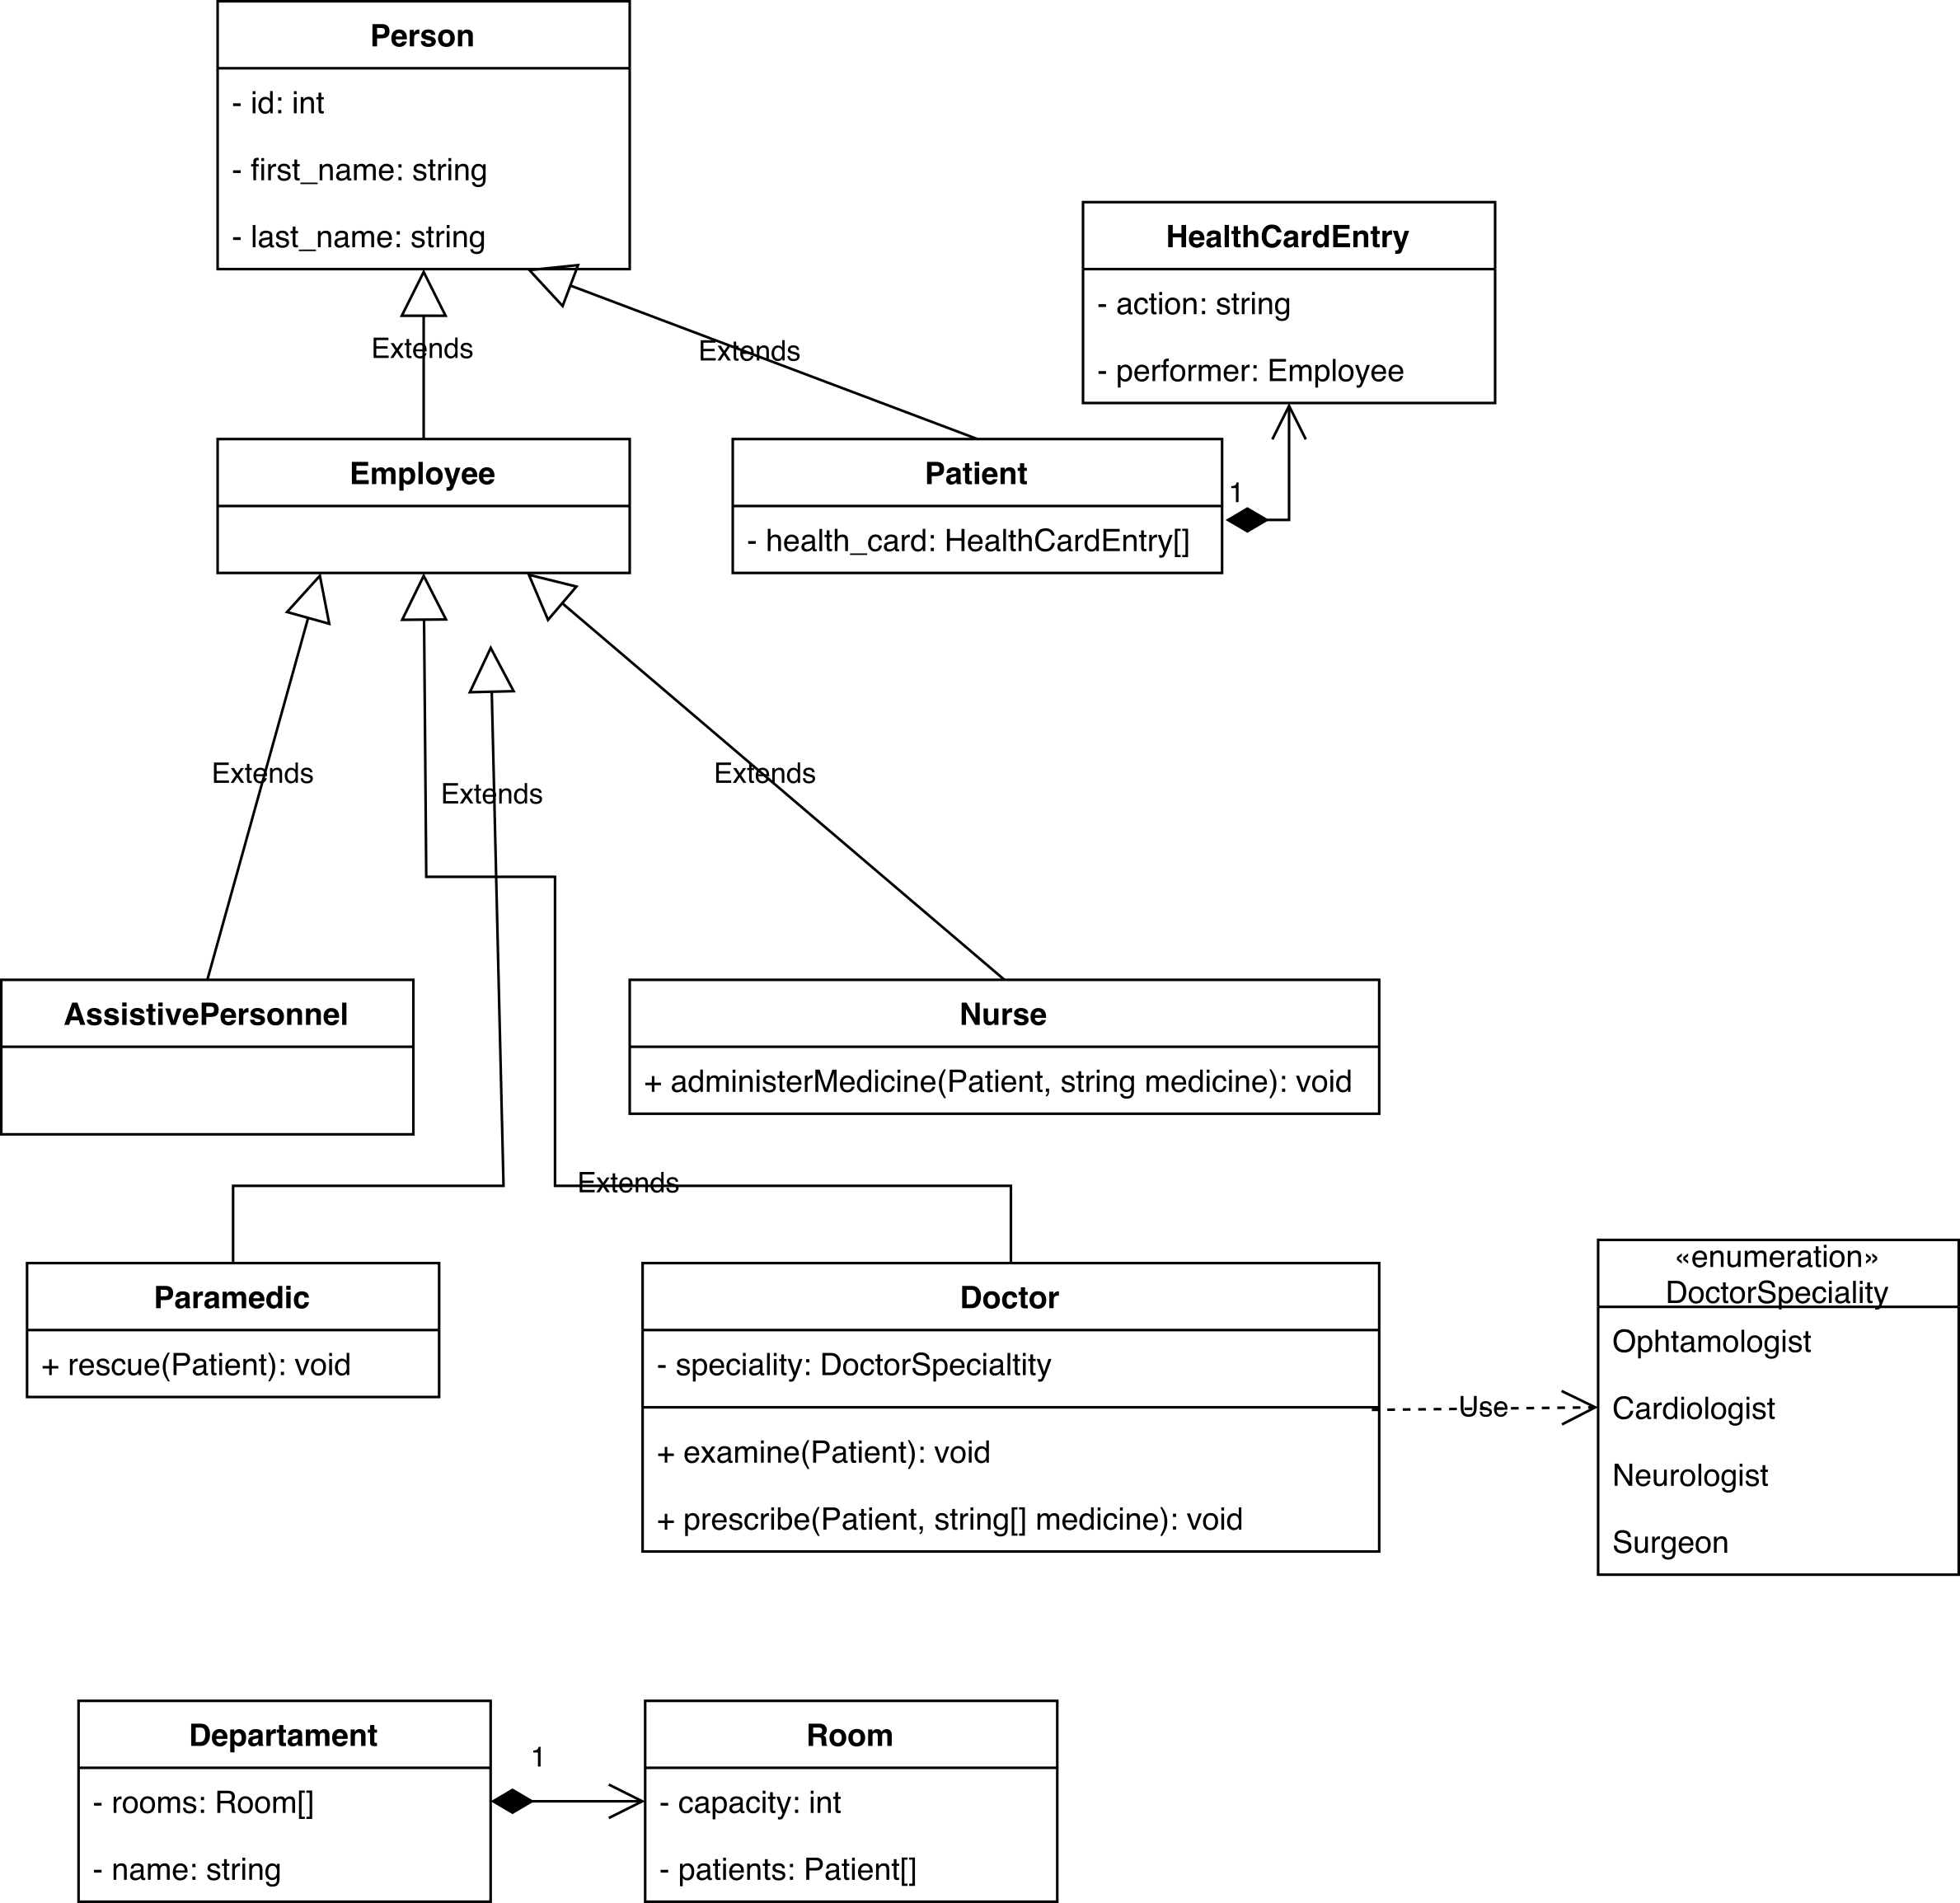
\includegraphics[width=\textwidth]{domain_model.png}
        \caption{Model danych projektu}
        \label{fig:data_model}
    \end{figure}
    \begin{figure}
        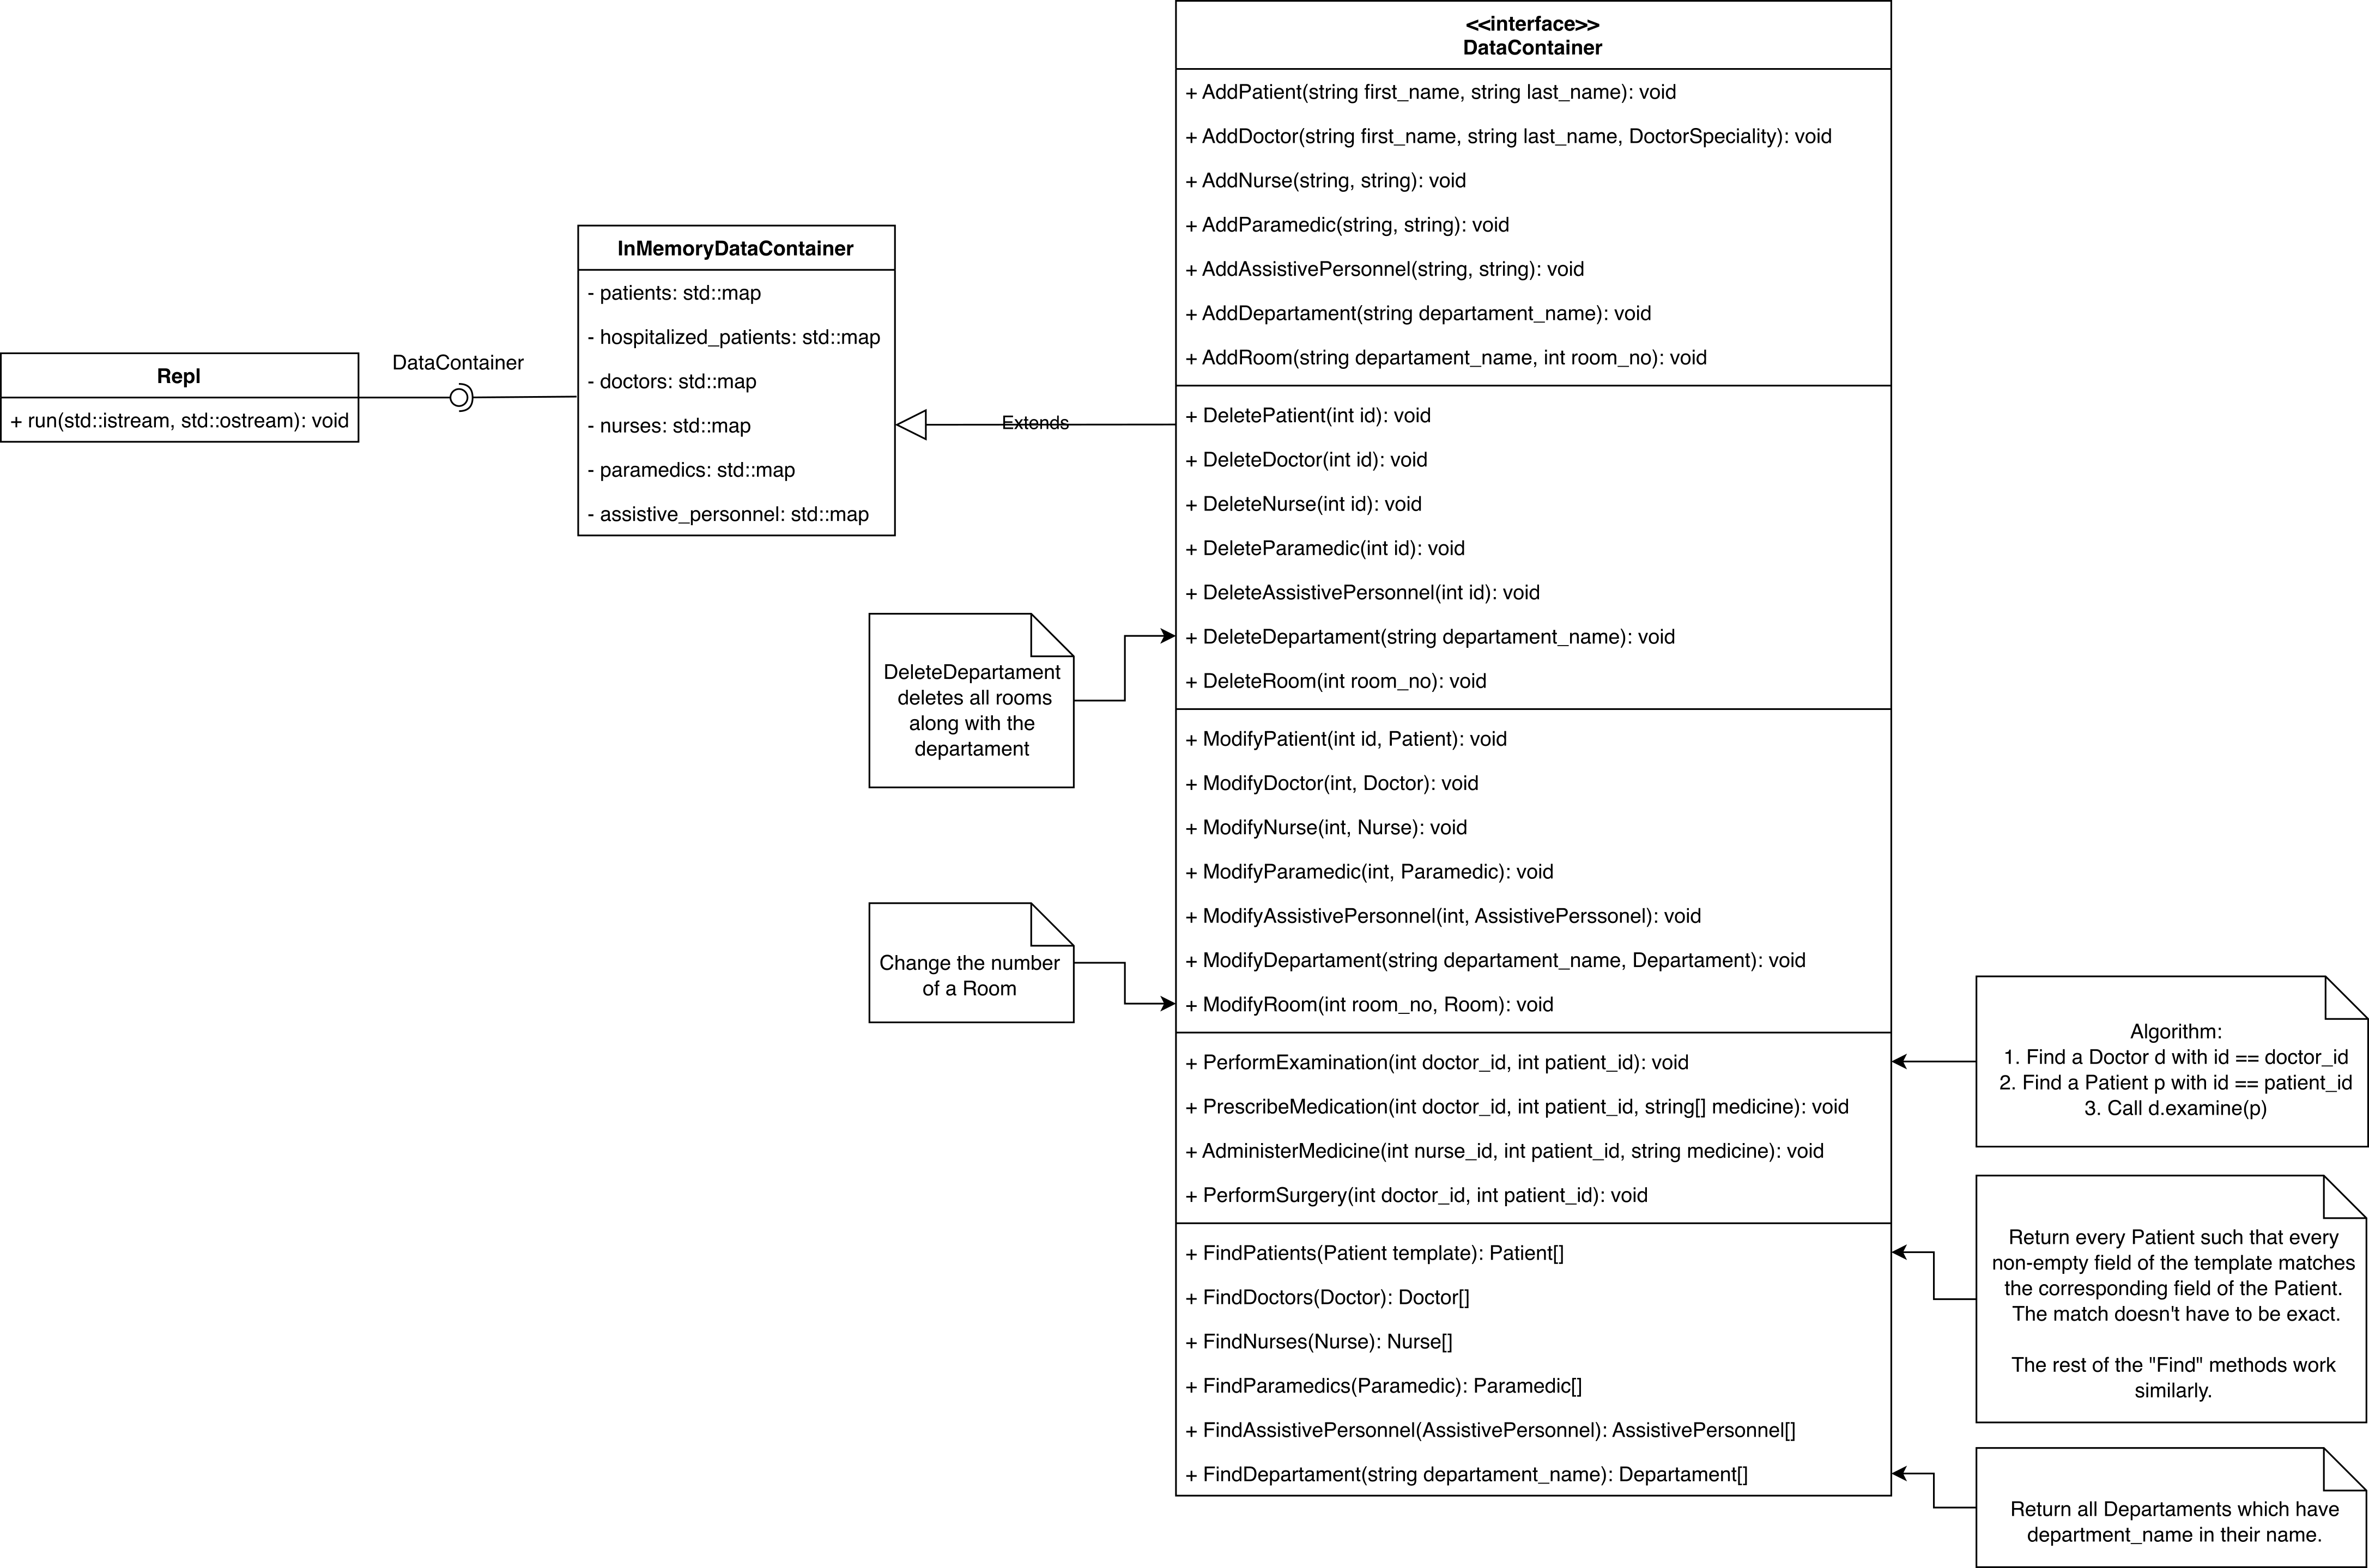
\includegraphics[width=\textwidth]{program_structure.png}
        \caption{Struktura projektu}
        \label{fig:program_structure}
    \end{figure}

\section{Polecenia REPL}
    Polecenia dzielą się na dwie kategorie:
    \begin{itemize}
        \item DML, oraz
        \item DQL.
    \end{itemize}
    Polecenia DML pozwalają na manipulowanie danymi, a polecenia DQL
    na odczytywanie danych. Polecenia DML dzielą się dodatkowo na:
    \begin{itemize}
        \item polecenia \texttt{add},
        \item polecenia \texttt{delete},
        \item polecenia \texttt{update},
        \item operacje dziedziny.
    \end{itemize}
    Przykłady poleceń przedstawiono na następujących listingach:
    \begin{itemize}
        \item Polecenia \texttt{add}: List.~\ref{list:add}.
        \item Polecenia \texttt{delete}: List.~\ref{list:delete}.
        \item Polecenia \texttt{update}: List.~\ref{list:update}.
        \item Operacje dziedziny: List.~\ref{list:domain}.
        \item Polecenia DQL: List.~\ref{list:DQL}.
    \end{itemize}
    \begin{listing}
        \begin{minted}{text}
add patient { first_name = <first_name>, last_name = <last_name> }
add doctor { first_name = <first_name>, last_name = <last_name>, speciality =
<doctor_speciality> }
add nurse { first_name = <first_name>, last_name = <last_name> }
add paramedic { first_name = <first_name>, last_name = <last_name> }
add assistive_personnel { first_name = <first_name>, last_name = <last_name> }
add departament { name = <departament_name> }
add room { departament = <departament_name>, room_no = <integer> }
        \end{minted}
        \caption{Polecenia \texttt{add}}
        \label{list:add}
    \end{listing}
    \begin{listing}
        \begin{minted}{text}
delete patient { id = <integer> }
delete doctor { id = <integer> }
delete nurse { id = <integer> }
delete paramedic { id = <integer> }
delete assistive_personnel { id = <integer> }
delete departament { departament = <departament_name> }
delete room { departament = <departament_name>, room_no = <integer> }
        \end{minted}
        \caption{Polecenia \texttt{delete}}
        \label{list:delete}
    \end{listing}
    \begin{listing}
        \begin{minted}{text}
update patient { id = <integer>
                 [, first_name = <first_name>]
                 [, last_name = <last_name>] }
update doctor { id = <integer>
                [, first_name = <first_name>]
                [, last_name = <last_name>]
                [, doctor_speciality = <doctor_speciality>] }
update nurse { id = <integer>
               [, first_name = <first_name>]
               [, last_name = <last_name>] }
update paramedic { id = <integer>
                   [, first_name = <first_name>]
                   [, last_name = <last_name>] }
update assistive_personnel { id = <integer>
                             [, first_name = <first_name>]
                             [, last_name = <last_name>] }
update departament { departament_name = <departament_name>,
                     new_name = <departament_name> }
update room { departament = <departament_name>,
              room = <integer>,
              new_no = <integer> }
        \end{minted}
        \caption{Polecenia \texttt{update}}
        \label{list:update}
    \end{listing}
    \begin{listing}
        \begin{minted}{text}
examine doctor { id = <integer> } patient { id = <integer> }
        | examine doctor { first_name = <first_name>, last_name = <last_name> }
                  patient { id = <integer> }
        | examine doctor { first_name = <first_name>, last_name = <last_name> }
                  patient { first_name = <first_name>, last_name = <last_name> }
prescribe doctor { id = <integer> }
               patient { id = <integer> }
               meds [ med1 [, med2][, med3][...] ]
administer nurse { id = <integer> }
               patient { id = <integer> }
               med <med1>
surgery doctor { id = <integer> } patient { id = <integer> }
        \end{minted}
        \caption{Operacje dziedziny}
        \label{list:domain}
    \end{listing}
    \begin{listing}
        \begin{minted}{text}
search patient {}
search doctor {}
search nurse {}
search paramedic {}
search assistant_personnel {}
search departament {}
        \end{minted}
        \caption{Polecenia DQL}
        \label{list:DQL}
    \end{listing}
\end{document}
